% utf-8, \n, 4 spaces
\documentclass{beamer}
\usepackage[utf8]{inputenc}
\usepackage[T1]{fontenc}
\usepackage{listings}
% textcomp enables upquote=true (= straight quotes) in lstset
\usepackage{textcomp}
\usepackage{pgf-umlcd}
\lstset{basicstyle=\ttfamily\footnotesize,breaklines=true,upquote=true,language=Java,keepspaces=true,numbers=left}

\usepackage{tikz}

\title{Funktionale Programmierung in Java}
\author[M. Klie]{Markus Klie}
\date[20.07.2022]{20. Juli 2022}

\begin{document}

\begin{frame}
    \titlepage
\end{frame}

\begin{frame}
\frametitle{\insertpagenumber}
Problemstellung 1: Sind das gültige Kreditkartennummern\footnotemark?
\begin{itemize}
\item 5555555555554444
\item 5105 1051 0510 5100
\item 4111-1111-1111-1111
\item 378282246310005
\end{itemize}

\footnotetext[1]{Es handelt sich um für Testzwecke reservierte Nummern}
\end{frame}

\begin{frame}
\frametitle{\insertpagenumber}
Ansatz 1:
\begin{center}
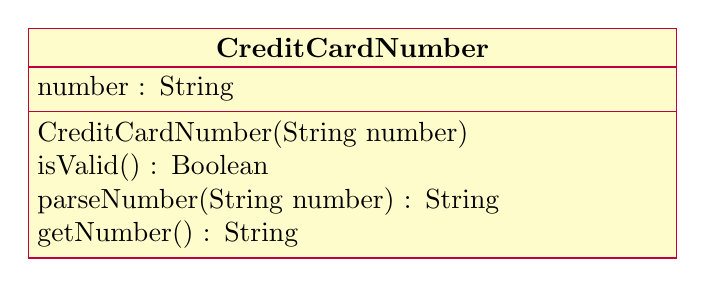
\begin{tikzpicture}
  \begin{class}[text width=8cm]{CreditCardNumber}{0,0}
    \attribute{number : String}

    \operation{CreditCardNumber(String number)}
    \operation{isValid() : Boolean}
    \operation{parseNumber(String number) : String}
    \operation{getNumber() : String}
  \end{class}
\end{tikzpicture}
\end{center}
\end{frame}

\begin{frame}[fragile]
\frametitle{\insertpagenumber}
\begin{lstlisting}
CreditCardNumber cc = new CreditCardNumber(candidate);
System.out.println(cc.getNumber());
System.out.println(cc.isValid());
\end{lstlisting}
\end{frame}

\begin{frame}
\frametitle{\insertpagenumber}
Problemstellung 2: Sind das gültige IMEI\footnotemark?
\begin{itemize}
    \item 35411809 746687 6
    \item 35411809 829642 1
    \item 99781729 757402 4
\end{itemize}
\footnotetext[2]{Es handelt sich um zufällig generierte Nummern}
\end{frame}

\begin{frame}
\frametitle{\insertpagenumber}
Ansatz 2a:
\begin{center}
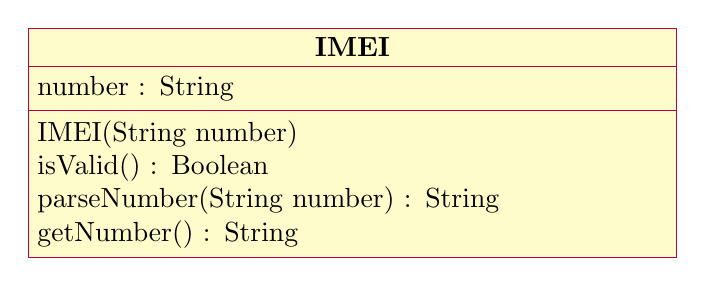
\begin{tikzpicture}
  \begin{class}[text width=8cm]{IMEI}{0,0}
    \attribute{number : String}

    \operation{IMEI(String number)}
    \operation{isValid() : Boolean}
    \operation{parseNumber(String number) : String}
    \operation{getNumber() : String}
  \end{class}
\end{tikzpicture}
\end{center}
\end{frame}

\begin{frame}[fragile]
\frametitle{\insertpagenumber}
\begin{lstlisting}
IMEI imei = new IMEI(candidate);
System.out.println(imei.getNumber());
System.out.println(imei.isValid());
\end{lstlisting}
\end{frame}

\begin{frame}
\frametitle{\insertpagenumber}
Ansatz 2b:
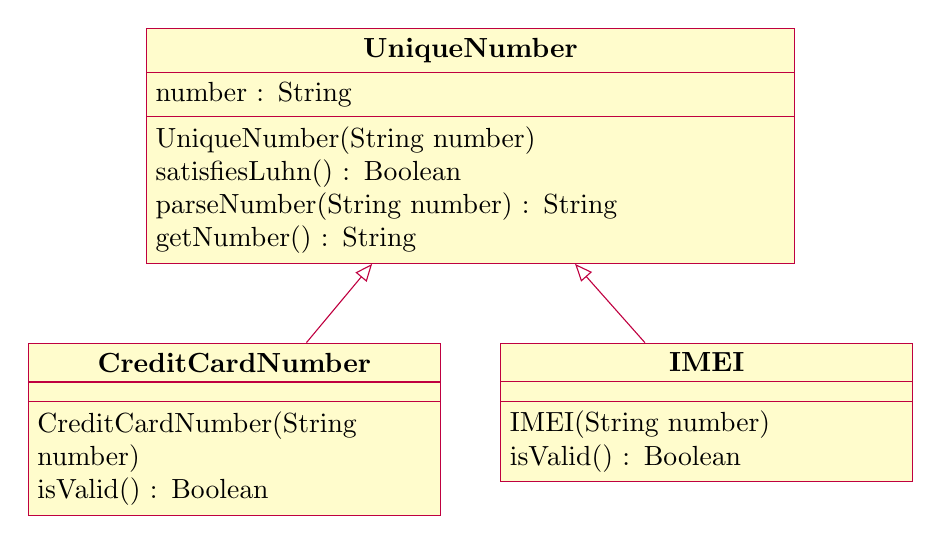
\begin{tikzpicture}
  \begin{class}[text width=8cm]{UniqueNumber}{0,0}
    \attribute{number : String}

    \operation{UniqueNumber(String number)}
    \operation{satisfiesLuhn() : Boolean}
    \operation{parseNumber(String number) : String}
    \operation{getNumber() : String}
  \end{class}

  \begin{class}[text width=5cm]{CreditCardNumber}{-3,-4}
    \inherit{UniqueNumber}

    \operation{CreditCardNumber(String number)}
    \operation{isValid() : Boolean}
  \end{class}

  \begin{class}[text width=5cm]{IMEI}{3,-4}
    \inherit{UniqueNumber}

    \operation{IMEI(String number)}
    \operation{isValid() : Boolean}
  \end{class}

\end{tikzpicture}

\end{frame}

\begin{frame}
\frametitle{\insertpagenumber}
Problemstellung 3: Kreditkartennummer oder IMEI?
\begin{itemize}
    \item 5555555555554444
    \item 5105105105105100
    \item 4111111111111111
    \item 378282246310005
    \item 354118097466876
    \item 354118098296421
    \item 997817297574024
\end{itemize}
\end{frame}

\begin{frame}
\frametitle{\insertpagenumber}
Moment mal \ldots
\begin{itemize}
    \item satisfiesLuhn (IMEI/CreditCardNumber)
    \item hasLength15 (IMEI/CreditCardNumber)
    \item hasLength16 (CreditCardNumber)
    \item hasValidCreditCardPrefix (CreditCardNumber)
\end{itemize}

\end{frame}

\begin{frame}
\frametitle{\insertpagenumber}
\begin{center}
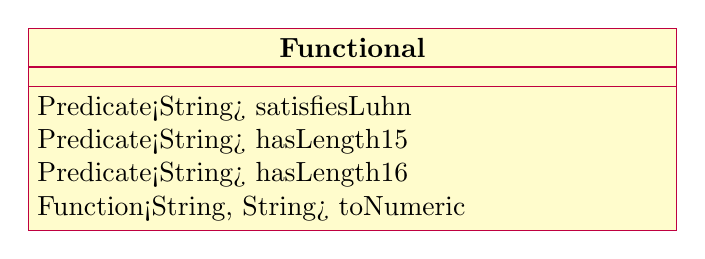
\begin{tikzpicture}
  \begin{class}[text width=8cm]{Functional}{0,0}
    \operation{Predicate<String> satisfiesLuhn}
    \operation{Predicate<String> hasLength15}
    \operation{Predicate<String> hasLength16}
    \operation{Function<String, String> toNumeric}
  \end{class}
\end{tikzpicture}
\end{center}
\end{frame}

\begin{frame}[fragile]
\frametitle{\insertpagenumber}
\begin{lstlisting}
Predicate<String> isCreditCardNumber = Functional
    .satisfiesLuhn
    .and(Functional.hasLength15
        .or(Functional.hasLength16))
    .and(Functional.hasValidCreditCardPrefix);

Predicate<String> isIMEI = Functional
    .satisfiesLuhn
    .and(Functional.hasLength15);

String parsed = Functional.toNumeric.apply(candidate);

System.out.println(parsed);
System.out.println(isCreditCardNumber.test(parsed));
System.out.println(isIMEI.test(parsed));
\end{lstlisting}
\end{frame}

\begin{frame}
\begin{quote}
Meditation guides the mind to grasp the reality as it is, without the abstractions created by our thoughts.
\end{quote}

\vspace{3cm}

-- Yehonathan Sharvit - in: Data-Oriented Programming (2022)
\end{frame}

\begin{frame}
\frametitle{Fragen}
\end{frame}

\end{document}
